\documentclass[12pt]{article}
\usepackage[utf8]{inputenc}
\usepackage[T1]{fontenc}
\usepackage[english]{babel}
\usepackage{amsmath, amssymb, amsthm}
\usepackage{geometry}
\usepackage{titling}
\usepackage{fancyhdr}
\usepackage{lipsum}
\usepackage{parskip}
\usepackage{forest}
\usepackage{tikz}
\usepackage{stmaryrd}
\usepackage{listings}
\usepackage{graphicx}
\usepackage{float}
\usepackage{subcaption}
\usepackage{csvsimple}

\geometry{top=4cm, bottom=4cm, left=4cm, right=4cm}
\pagestyle{fancy}
\fancyhf{}
\rhead{Pierre Pili $\cdot$ Marie Gardie $\cdot$ Isée Biglietti}
\lhead{Macroeconomics 1}
\cfoot{\thepage}

\title{MACROECONOMICS 1 - Problem Set 2}
\author{PILI Pierre $\cdot$ GARDIE Marie $\cdot$ BIGLIETTI Isée}
\date{\today}
\begin{document}
\maketitle
\section{Data Work}
\subsection{}
We used a data about France comming from the FRED website. To be able to respond to the questions of this exercise, we downloaded 6 time series: 
\begin{itemize}
    \item Real Gross Domestic Product for France (CLVMNACSCAB1GQFR), in millions of 2010 euros.
    \item Private Final Consumption Expenditure for France (NAEXKP02FRQ189S), in 2010 euros.
    \item Gross Fixed Capital Formation for France (NAEXKP04FRQ189S), in 2010 euros.
    \item Average Annual Hours Worked by Persons Engaged for France (AVHWPEFRA065NRUG), in hours.
    \item Employment in France (FRAEMPT), in millions of people.
    \item Total population for France (POPTOTFRA647NWDB), in persons.
\end{itemize}
We used those times series to derive the private final consumption and gross fixed capital formation per capita.
We used employment data as well as average annual hours worked by persons engaged and total population to obtain per capita hours worked. 
Therefore, we obtained a joint dataframe with our 5 variables of ineterest: Year, and Investment, Consumption, Hours Worked and GDP, all per capita.
The regressions we computed on the log of variables gives the expected trends as seen in class for the US economy (See figure \ref{fig:descriptive}).
We then decomposed the different signals applying an HP-filter and plotted their cyclical components on the same graph (See figure \ref{fig:cycles}).
We observe that cyclical components are moving in the same direction over time, meaning that the variables at play are procyclical.
Those results corresponds to what we have seen in class for the US economy.
Though, this graphical decomposition doesn't enable us to precisly compare the volatility of GDP, consumption and hours worked. We then need to compute quantitatively indicators in order to derive some conclusions.

\subsection{}
\begin{table}[h]
  \centering
  \begin{tabular}{|c|c|c|c|c|}
      \hline
      & GDP & Investment & Consumption & Hours Worked \\
      \hline
      Correlation with GDP & 1 & 0.94 & 0.89 & 0.77 \\
      \hline
      Standard Deviation & 0.016 & 0.05 & 0.015 & 0.016 \\
      \hline
  \end{tabular}
  \caption{Correlation and Relative Standard Deviation with Respect to GDP}
\end{table}

First of all, we had that consumption, investment and hours worked were strongly procyclical for the US. 
Observing that all of our correlation coeficient with GDP are positives and close to $1$, we can enforce the same conclusion for these $3$ variables, with consumption and investment being even more procyclical.
\newline    
Second of all, we saw that for the US, consumption was less volatile than GDP, whereas investment was more. Regarding hours worked, it was as volitile as GDP
Using the standard deviation reported in the table above, we have that $\sigma_Y > \sigma_C$, $\sigma_Y < \sigma_I$ and $\sigma_Y = \sigma_H$ for France. So we found exactly the same results as what we saw in the lecture for the case of the US economy!

\begin{figure}
    \centering
    \begin{subfigure}[b]{1\textwidth}
        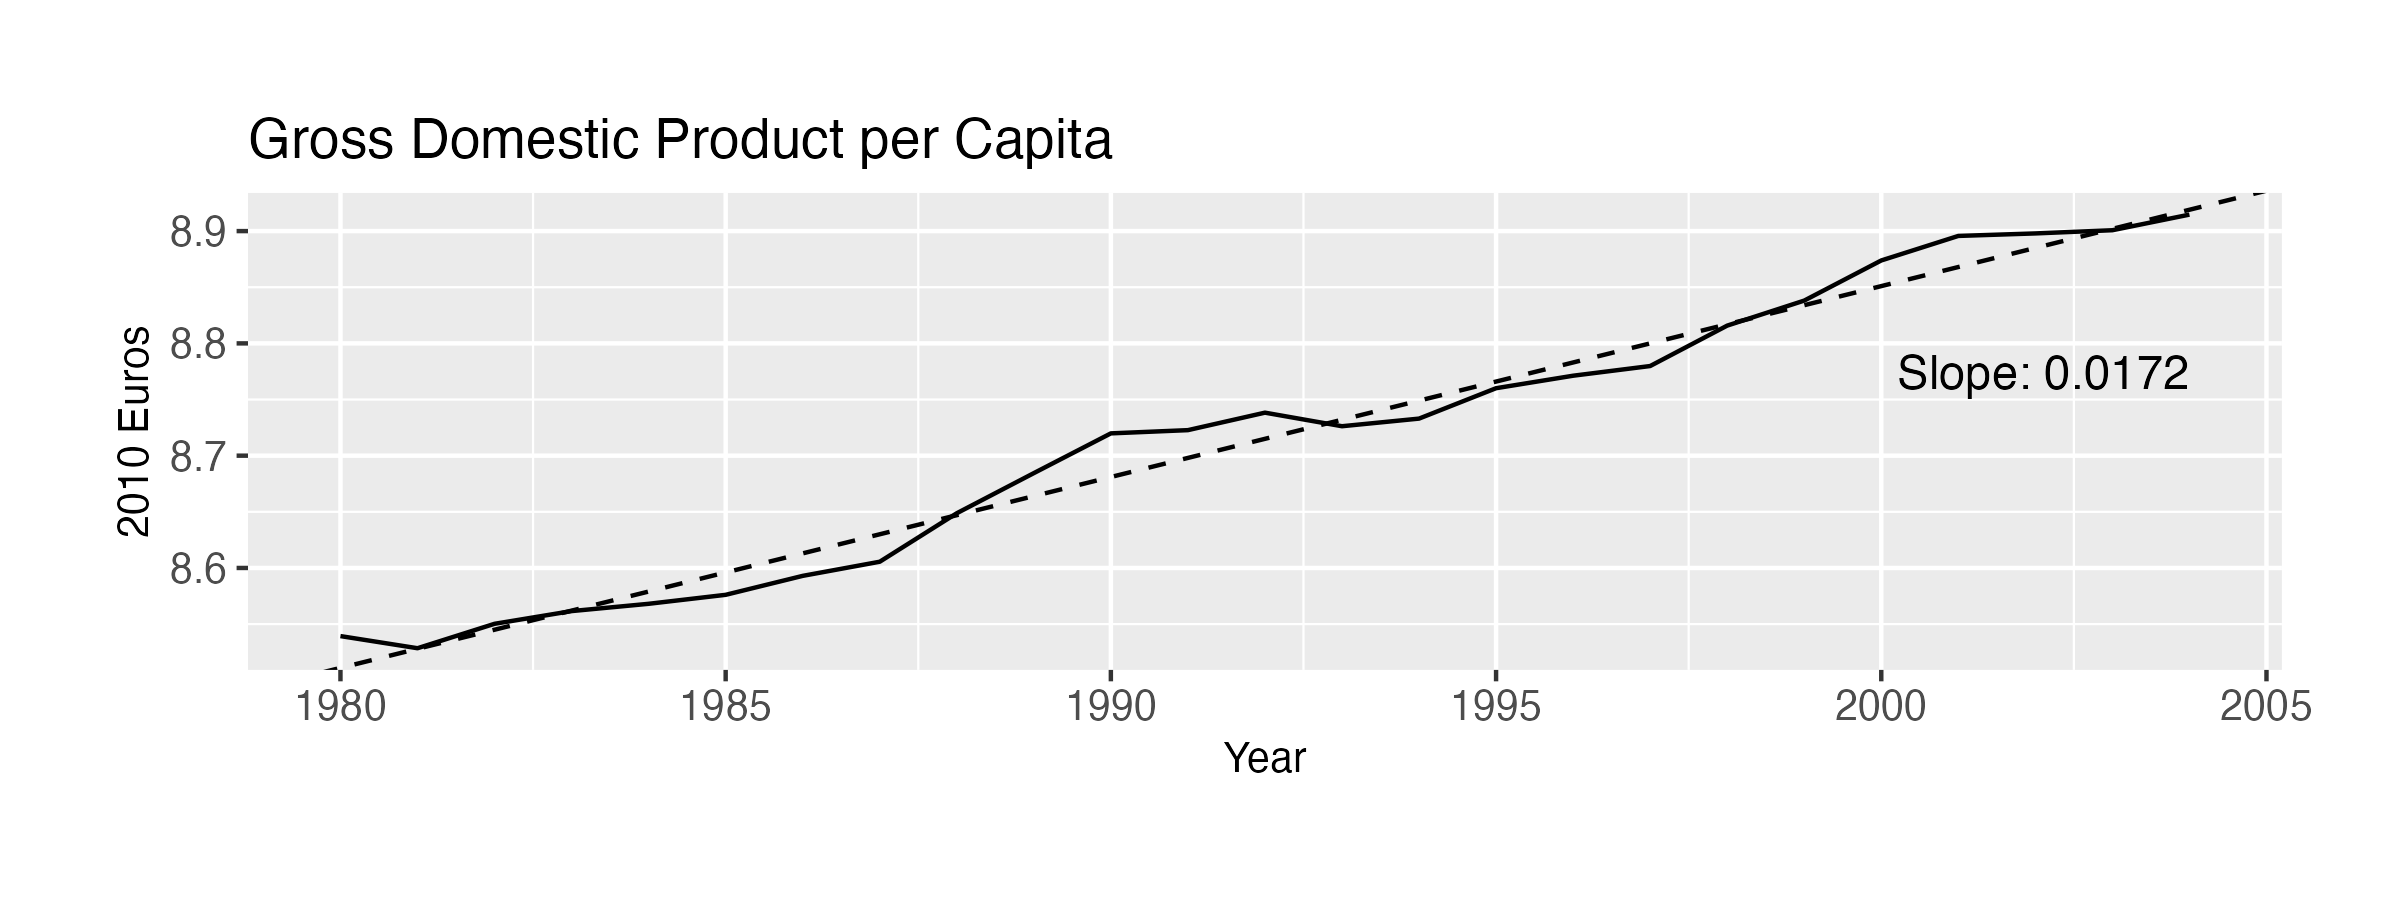
\includegraphics[width=\textwidth]{OUTPUT/MEDIA/loggdp_pc.png}
    \end{subfigure}
    \vspace{-20pt}
    \begin{subfigure}[b]{1\textwidth}
        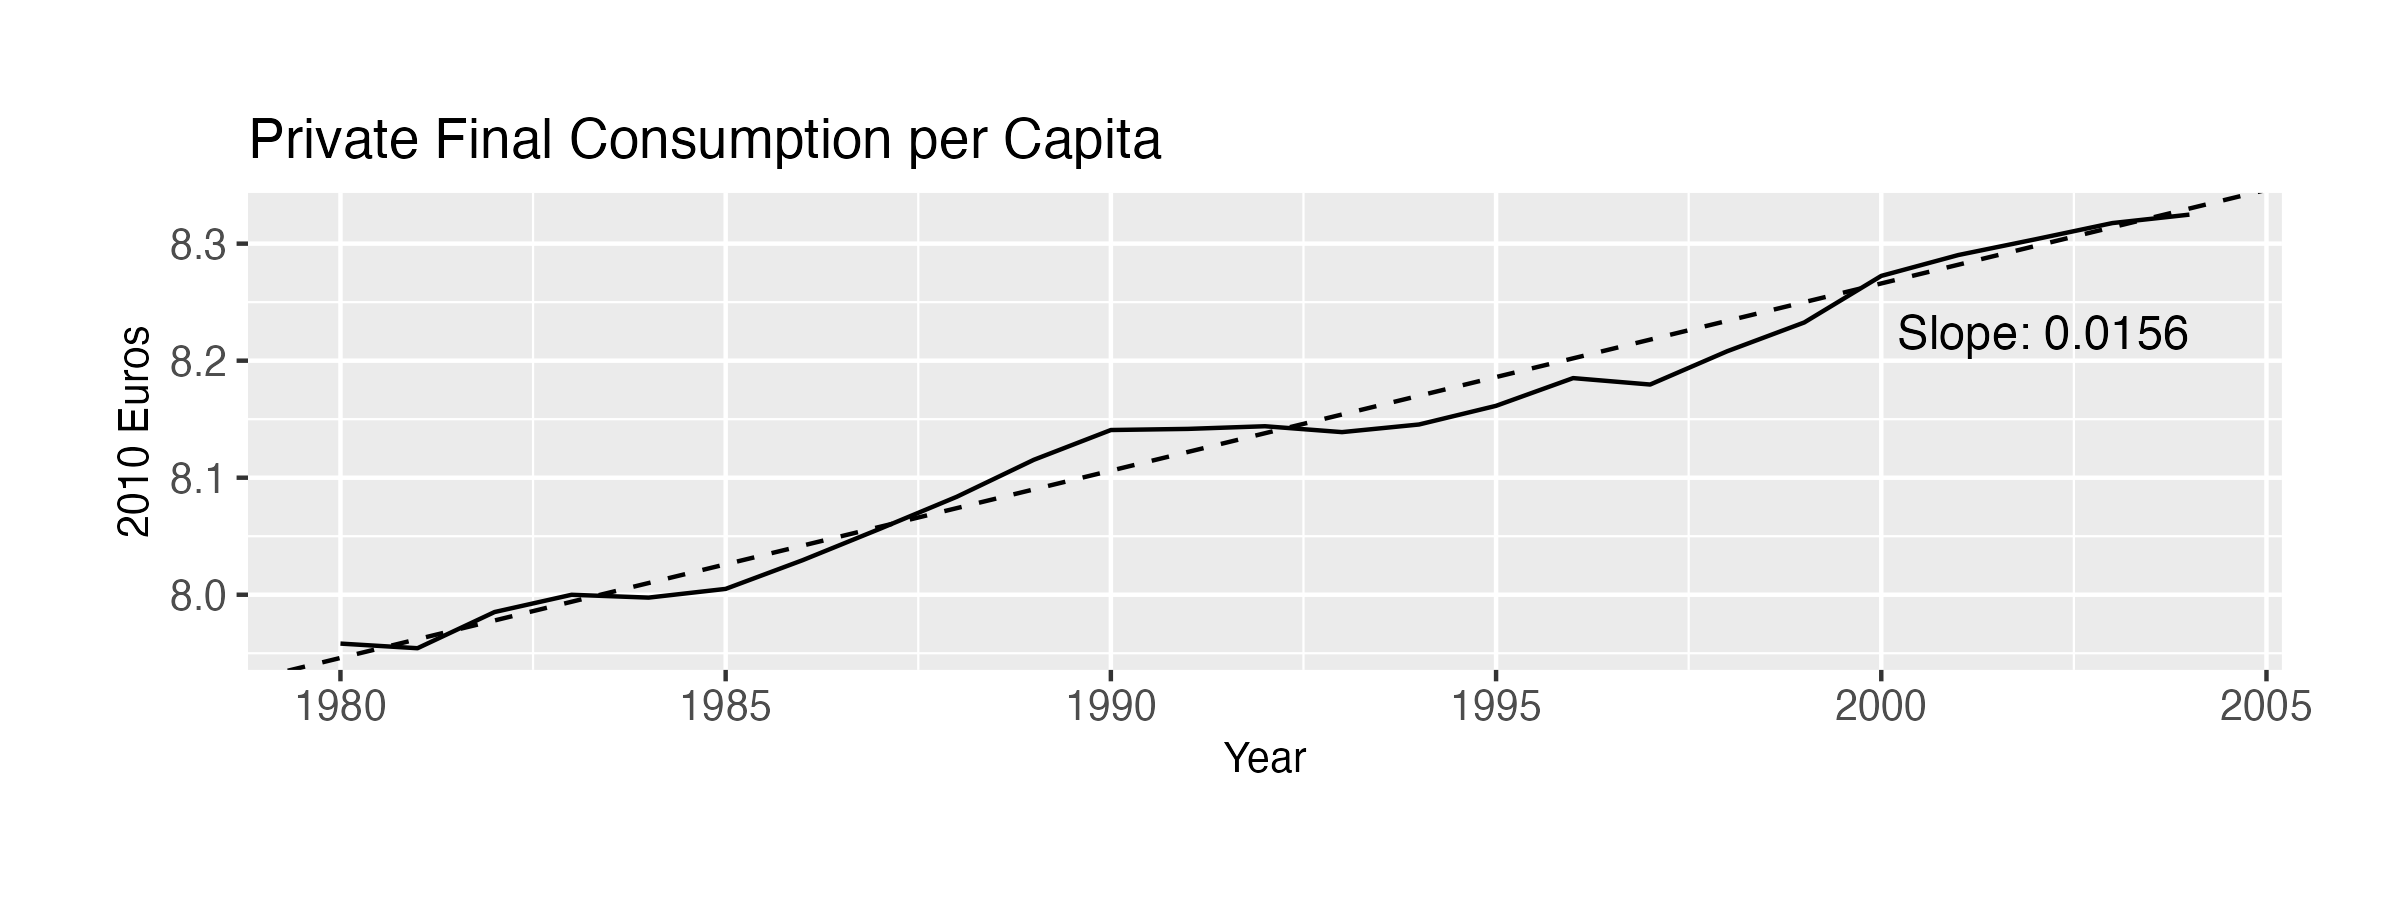
\includegraphics[width=\textwidth]{OUTPUT/MEDIA/logcons_pc.png}
    \end{subfigure}
    \vspace{-20pt}
    \begin{subfigure}[b]{1\textwidth}
        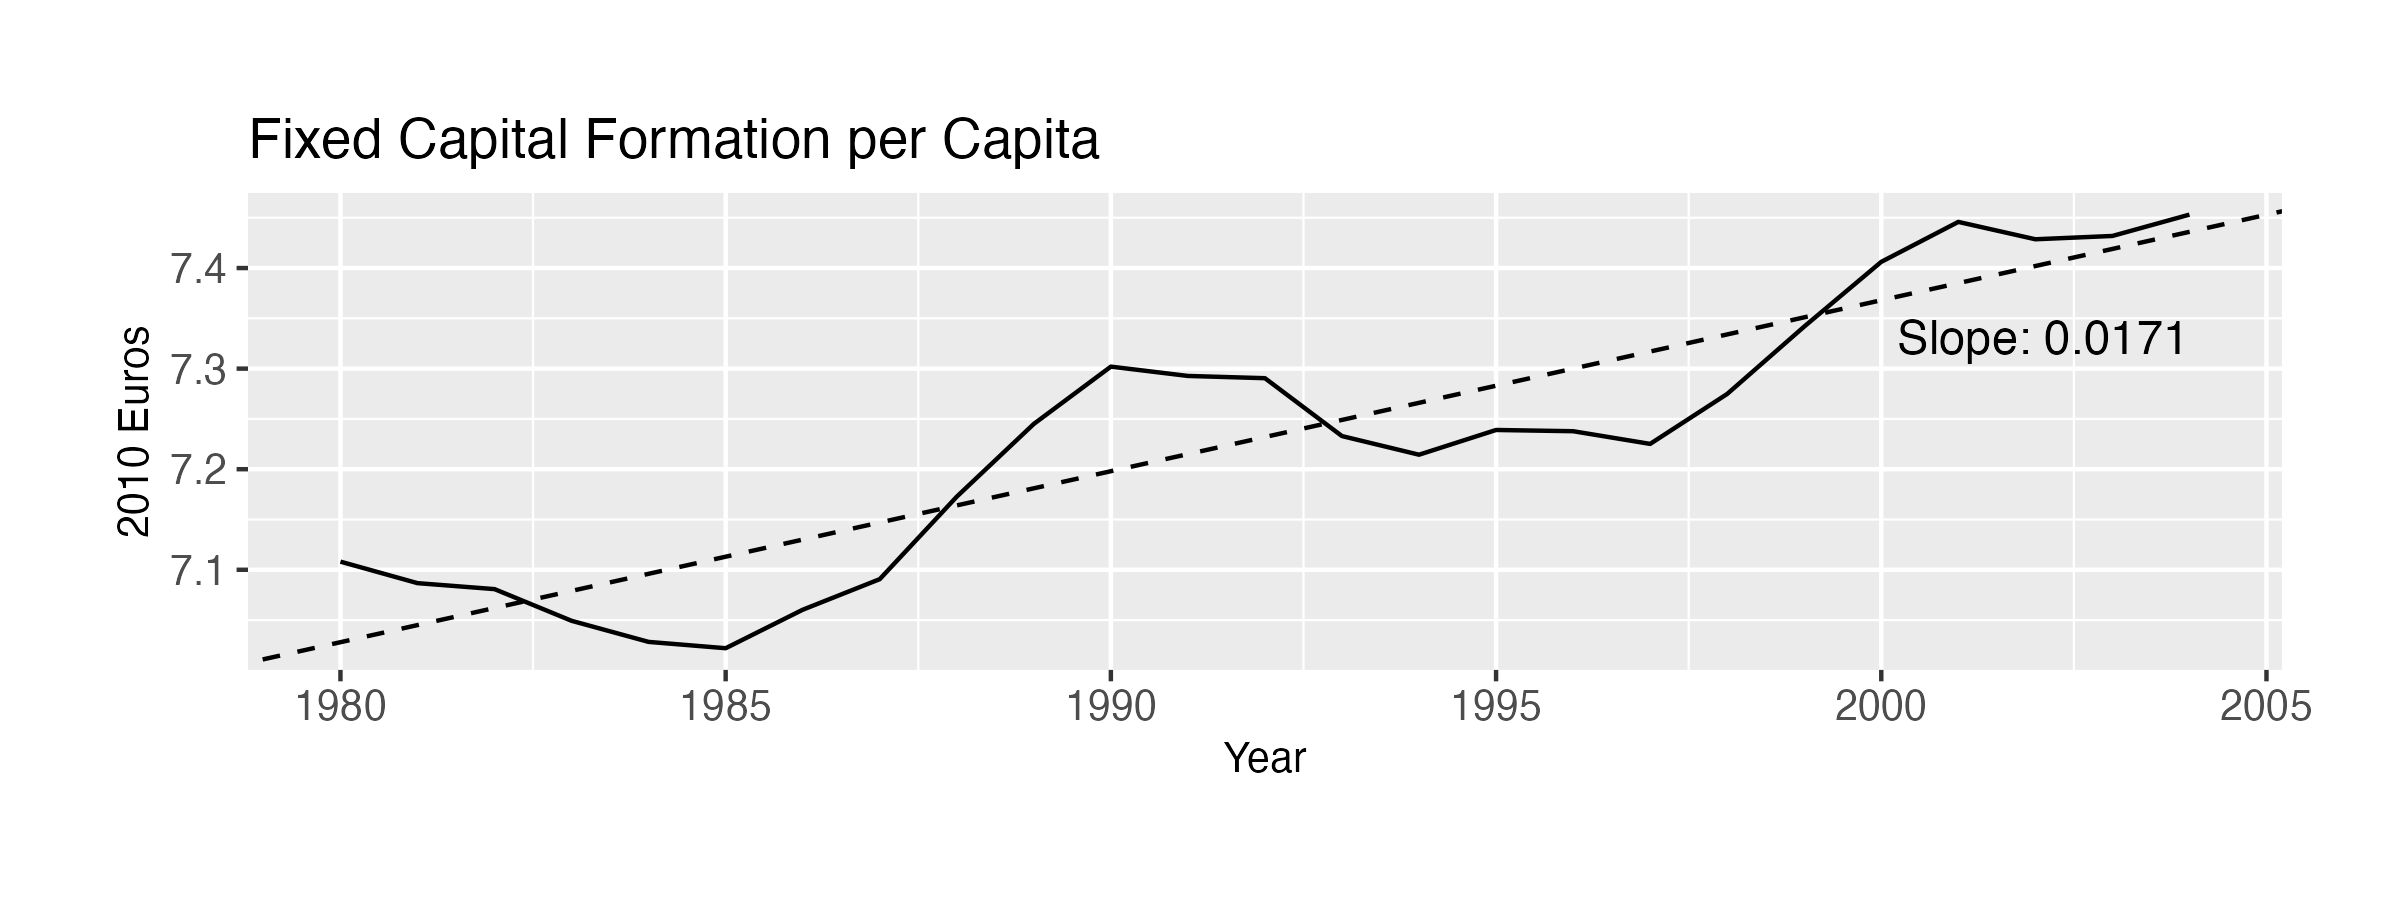
\includegraphics[width=\textwidth]{OUTPUT/MEDIA/loginv_pc.png}
    \end{subfigure}
    \vspace{-20pt}
    \begin{subfigure}[b]{1\textwidth}
        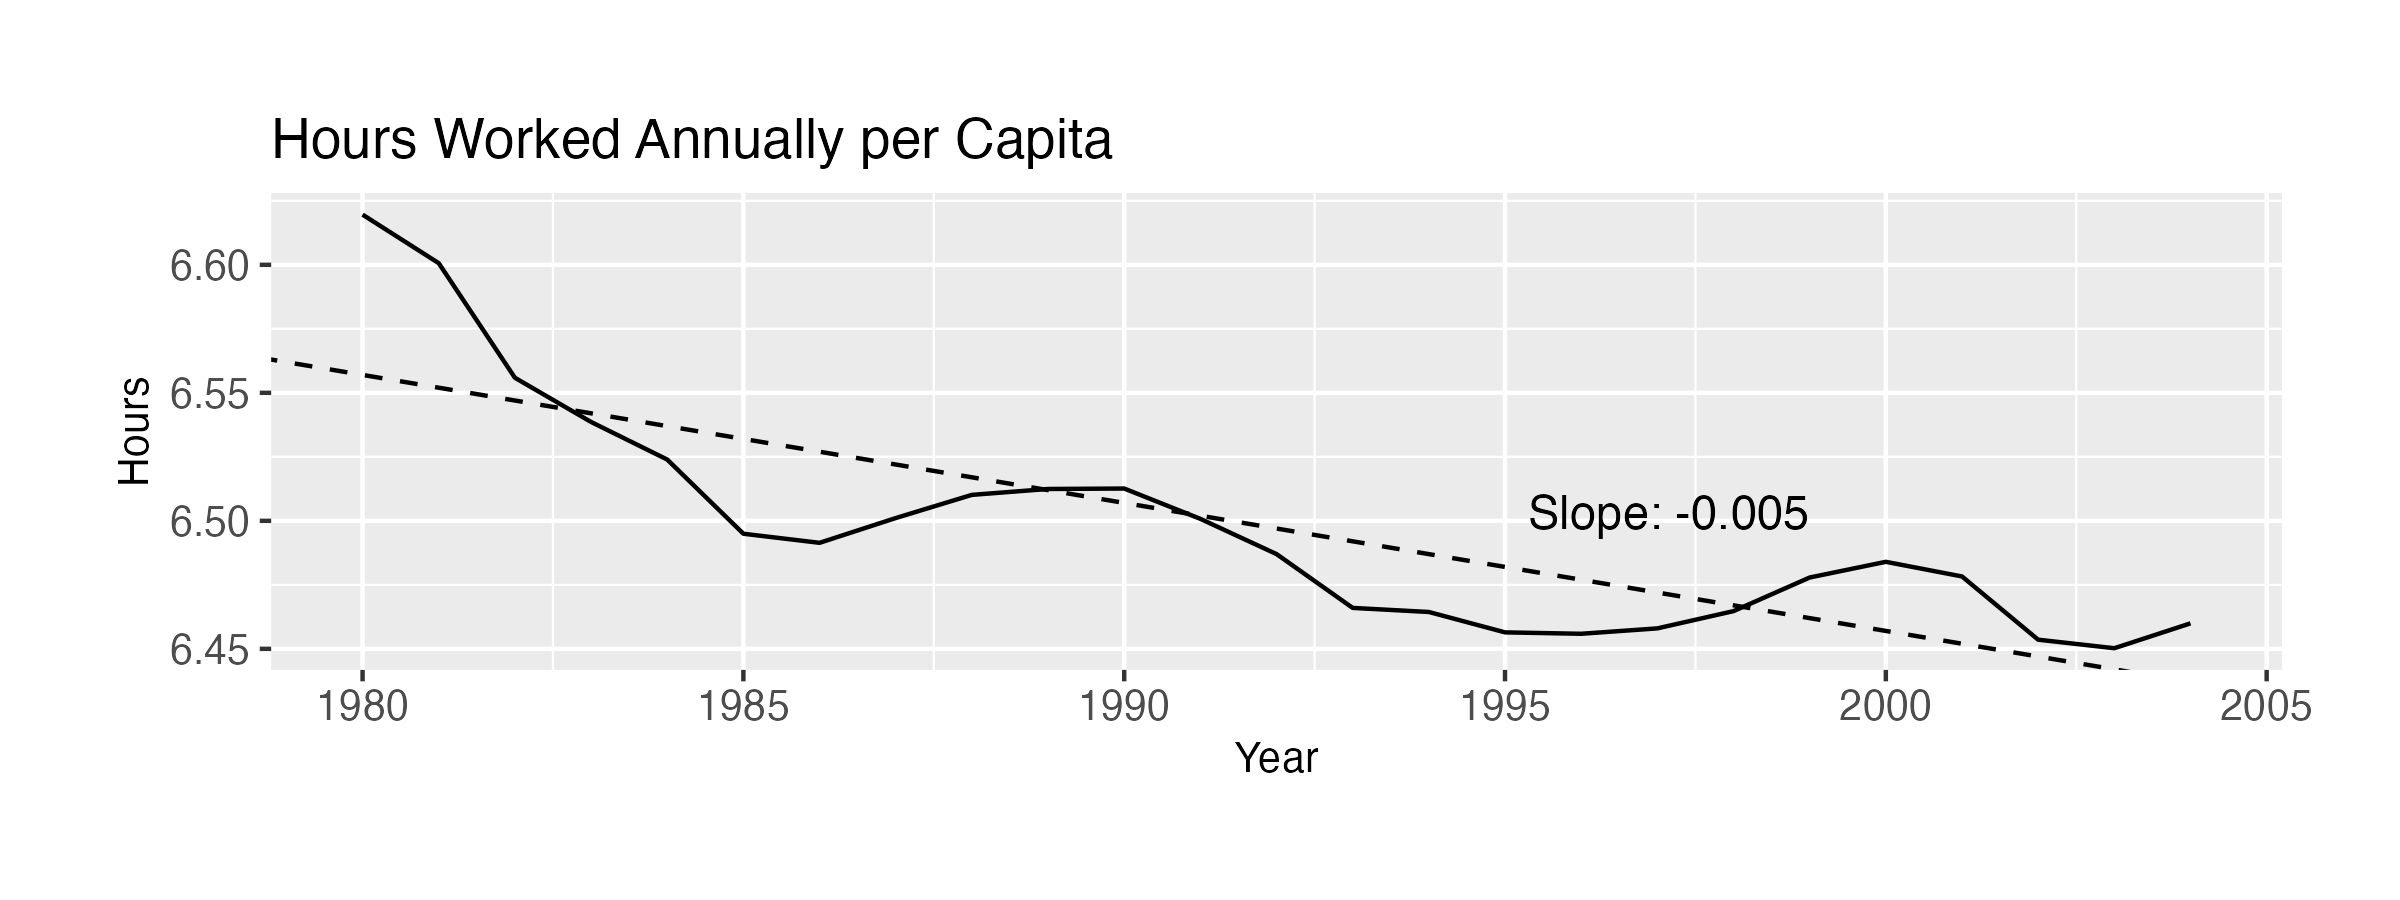
\includegraphics[width=\textwidth]{OUTPUT/MEDIA/loghours_pc.png}
    \end{subfigure}
    \caption{GDP, Consumption, Investment and Hours Worked per Capita}
    \label{fig:descriptive}
\end{figure}
\clearpage % Ajoute une page vide après l'image

\begin{figure}[h]
    \centering
    \hspace{-20pt}
    \begin{tikzpicture}[baseline=(current bounding box.center)]
        \node at (0,0) {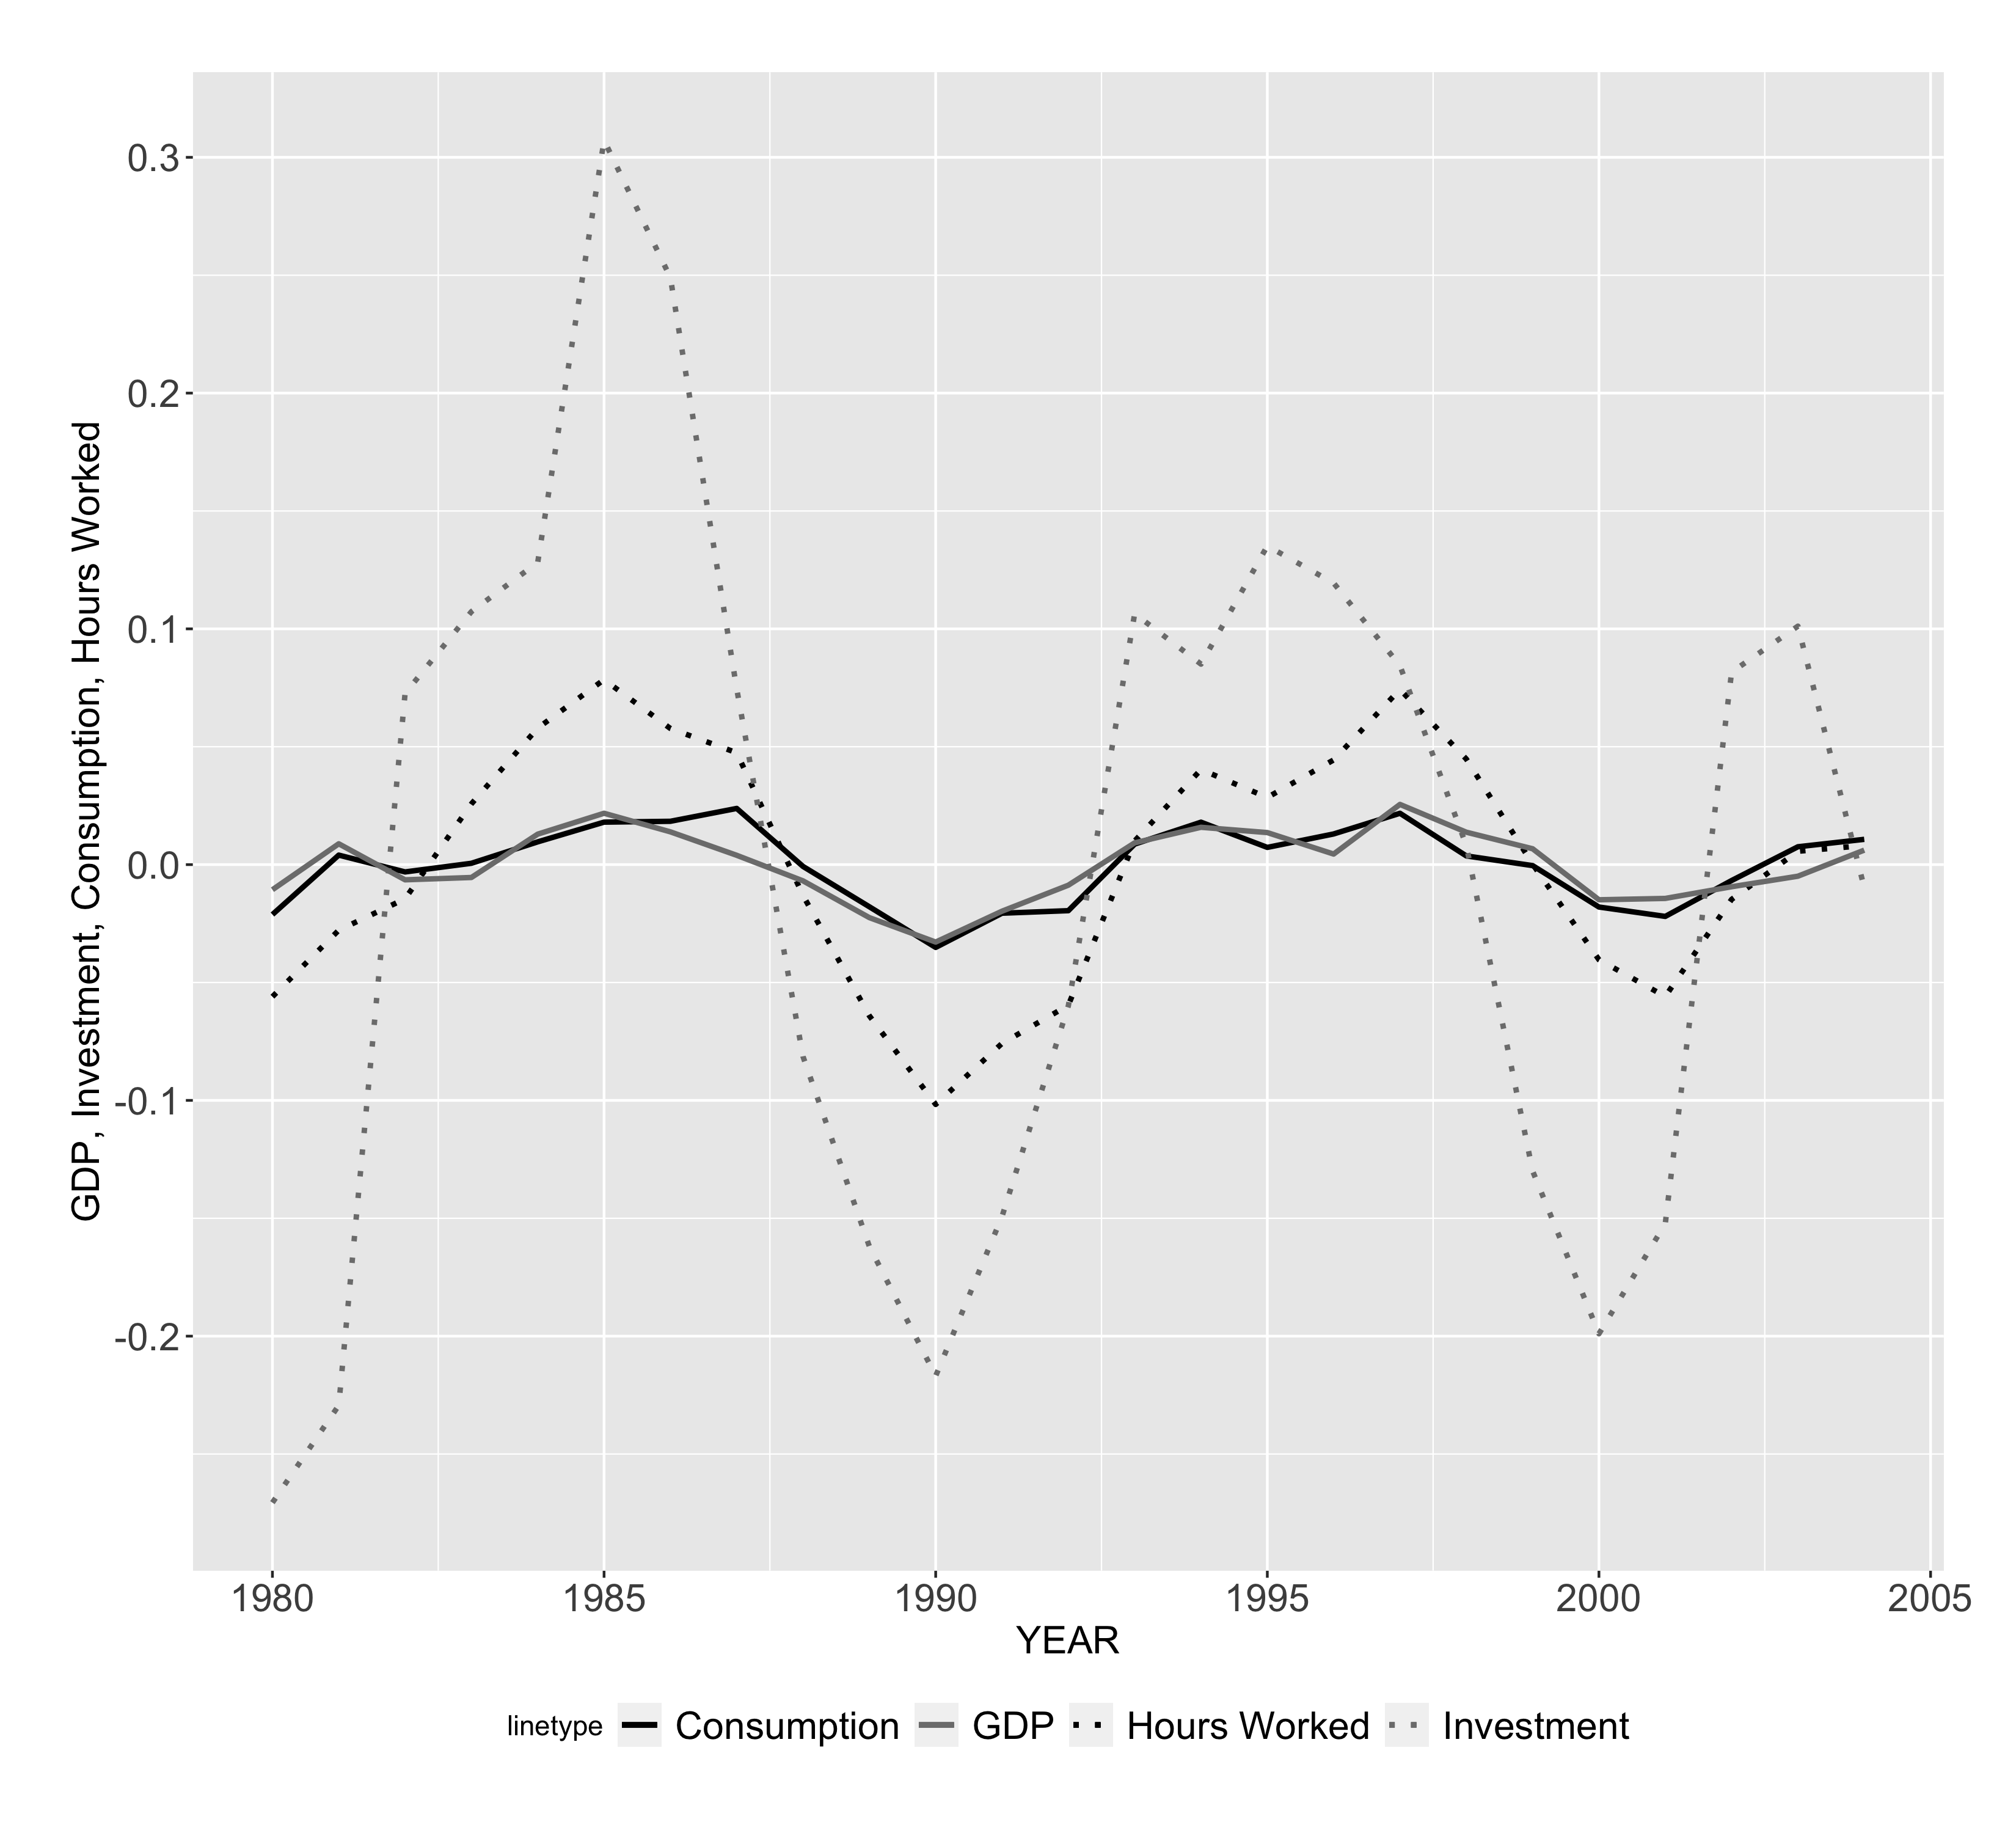
\includegraphics[width=1\textwidth]{OUTPUT/MEDIA/cycles.png}};
    \end{tikzpicture}
    \caption{Cyclical compenents in HP decomposition for GDP, Consumption Investment and Hours Worked per Capita}
    \label{fig:cycles}
\end{figure}
\newpage
\section{A Simple model of business cycles}
\subsubsection*{Notations}
In the following, we will use freely the notations below :
\begin{itemize}
    \item $Y_t = F(K_t, L_t) = A_t K_t^{\alpha}(1 - L_t)^{1 - \alpha}$
    \item $w_t = A_t K_t^{\alpha} (1 - \alpha)(1 - L_t)^{-\alpha} = - F_L(K_t,L_t)$
    \item $R_t = \alpha A_t K_t^{\alpha -1 } (1 - L_t)^{1 - \alpha} + 1 - \delta = F_K(K_t, L_t) + 1 - \delta$
\end{itemize}


\subsection{}
The lagrangian of the maximization problem writes :
\begin{equation*}
    \mathcal{L}(C_t,L_t,K_{t+1}) = \mathbb{E}_0\sum_{t=0}^{\infty} \Big[ \beta^t (\ln C_t + v(L_t)) + \lambda_t (F(K_t, L_t) + (1 - \delta)K_t - C_t - K_{t+1}) \Big]
\end{equation*}
Deriving the associated FOCs for $t \in \mathbb{N}$ viewed from date $t$:
\[
\begin{cases}
    \begin{array}{@{}l}
        \displaystyle \frac{\partial \mathcal{L}}{\partial C_t} =  \frac{\beta^t}{C_t} - \lambda_t = 0\\[12pt]
        \displaystyle \frac{\partial \mathcal{L}}{\partial L_t} = \beta^t v'(L_t) - \lambda_t w_t = 0\\[12pt]
        \displaystyle \frac{\partial \mathcal{L}}{\partial K_{t+1}} = \mathbb{E}_t \left( \lambda_{t+1} R_{t+1} \right) - \lambda_t = 0\\
    \end{array}
\end{cases}
\Longleftrightarrow \quad
\begin{cases}
    \begin{array}{@{}l}
        \displaystyle \frac{\beta^t}{C_t} = \lambda_t\\[12pt]
        \displaystyle \beta^t v'(L_t) = \lambda_t w_t\\[12pt]
        \displaystyle \mathbb{E}_t \left( \lambda_{t+1} R_{t+1} \right) = \lambda_t\\
    \end{array}
\end{cases}
\]
Inserting the expressions of $\lambda_t$ and $\lambda_{t+1}$ from the first equation, one gets the Euler intertemporal equation: 
\begin{equation*}
    \mathbb{E}_t \left( \frac{\beta^{t+1}}{C_{t+1}} R_{t+1} \right) = \frac{\beta^t}{C_t}
\end{equation*}
Which implies : 
\begin{equation*}
   \beta~\mathbb{E}_t \left( \frac{C_t}{C_{t+1}} R_{t+1} \right) = 1
\end{equation*}


\subsection{}
With $\delta = 1$, the Euler Equation becomes: 
\begin{equation*}
   \beta~\mathbb{E}_t \left( \frac{C_t}{C_{t+1}} F_K(K_{t+1}, L_{t+1}) \right) = 1
\end{equation*}
Using that $C_t = (1 - s_t) Y_t$, and assuming a constant saving ratio $s$: 
\begin{equation*}
   \beta~\mathbb{E}_t \left( \frac{(1 - s)Y_t}{(1-s)Y_{t+1}}  F_K(K_{t+1}, L_{t+1}) \right) = 1
\end{equation*}
Which implies :
\begin{equation*}
   \beta~\mathbb{E}_t \left( \frac{Y_t}{Y_{t+1}} A_{t+1} \alpha K_{t+1}^{\alpha - 1} (1 - L_{t+1})^{1 - \alpha} \right) = 1
\end{equation*}
Yet, $\displaystyle \frac{Y_{t+1}}{K_{t+1}}= A_{t+1} K_{t+1}^{\alpha-1} (1 - L_{t+1})^{1 - \alpha}$. 
Thus, one gets:
\begin{alignat*}{2}
    1   &= \alpha \beta~\mathbb{E}_t\frac{Y_t}{Y_{t+1}} \frac{Y_{t+1}}{K_{t+1}} \quad\\
        &= \alpha \beta~\mathbb{E}_t \frac{Y_t}{K_{t+1}} \quad\\
        &= \alpha \beta~\mathbb{E}_t \frac{Y_t}{sY_t} \quad\\
        &= \frac{\alpha \beta}{s} \quad
\end{alignat*}
Which yields $s = \alpha \beta$.\newline\newline
This constant saving rate was deducted from the first and third equation of the system, which means that a solution with a constant saving rate complies with the Euler's equation. It is clear that the law of motion of capital is also verified under a constant saving rate. Thus, the constant saving rate solves the planners' problem under the condition that the intratemporal condition can be verified.\newline
Using the first and the second first order conditions to derive the intratemporal condition:
\begin{alignat*}{2}
    v'(L_t) &= \frac{w_t}{C_t} \quad\\
            &= \frac{w_t}{(1-\alpha \beta)F(K_t, L_t)}
\end{alignat*}
Simplifying,
\begin{equation*}
    g(L_t) \equiv (1-L_t)v'(L_t) = \frac{1 - \alpha}{1 - \alpha \beta}
\end{equation*}
Assuming that $v$ is a well behaved periodic utility function with decreasing marginal utility of leisure, the previous equation has a unique solution in $L_t$ and $s$ thus solves the planner's maximization problem. Indeed, $L \equiv g^{-1}\left( \frac{1 - \alpha}{1 - \alpha \beta} \right)$ is well defined and unique as $g$ is decreasing on $(0, 1]$.\newline
A constant saving rate implies a constant labor supply of $N = 1 - L$.



\subsection{}
As the constant saving rate is equal to $\alpha \beta $, consumption is clearly procyclical as experienced in reality since: 
\begin{equation*}
    \frac{\partial Y_t}{\partial C_t} = \frac{1}{1 - \alpha \beta} > 0
\end{equation*}
Similarly, investment is procyclical and matches reality since $I_t = K_{t+1} = \alpha \beta Y_t$ and so:
\begin{equation*}
    \frac{\partial Y_t}{\partial I_t} = \frac{1}{\alpha \beta} > 0
\end{equation*}
However, as $w_t = v'(L)C_t$, an increase in wages implies a proportional increase in consumption but leisure and labor supply remain unchanged (see 2.2). Thus, in this simplified model, the stylised facts on working hours are not verified: indeed, employment and hours are observed strongly procyclical.  

\section{Savings rates in the Ramsey model}
\subsubsection*{Notations}
As in the previous section, we will use freely the results and notations below~:
\begin{itemize}
    \item $Y_t = F(K_t, L_t) = A_t K_t^{\alpha}$
    \item $\displaystyle R_t = \alpha A_t K_t^{\alpha -1 } = F_K(K_t, L_t) = \alpha \frac{Y_t}{K_t}$
\end{itemize}
\subsection{}
In this question we assume $\sigma \not= 1$.
The lagrangian of the maximization problem writes :
\begin{equation*}
    \mathcal{L}(C_t,L_t,K_{t+1}) = \mathbb{E}_0\sum_{t=0}^{\infty} \left[ \beta^t \frac{C_t^{1-\sigma} - 1}{1-\sigma} + \lambda_t \Big( F(K_t, L_t) - C_t - K_{t+1} \Big) \right]
\end{equation*}
Deriving the associated FOCs for $t \in \mathbb{N}$ viewed from date $t$:
\[
\begin{cases}
    \begin{array}{@{}l}
        \displaystyle \frac{\partial \mathcal{L}}{\partial C_t} =  \frac{\beta^t}{C_t^{\sigma}} - \lambda_t = 0\\[12pt]
        \displaystyle \frac{\partial \mathcal{L}}{\partial K_{t+1}} = \mathbb{E}_t \left( \lambda_{t+1} R_{t+1} \right) - \lambda_t = 0\\
    \end{array}
\end{cases}
\Longleftrightarrow \quad
\begin{cases}
    \begin{array}{@{}l}
        \displaystyle \frac{\beta^t}{C_t^{\sigma}} = \lambda_t\\[12pt]
        \displaystyle \mathbb{E}_t \left( \lambda_{t+1} R_{t+1} \right) = \lambda_t\\
    \end{array}
\end{cases}
\]
Inserting the expressions of $\lambda_t$ and $\lambda_{t+1}$ from the first equation, one gets the Euler intertemporal equation: 
\begin{equation*}
   \beta~\mathbb{E}_t \left[ \left( \frac{C_t}{C_{t+1}} \right)^{\sigma} R_{t+1} \right] = 1
\end{equation*}
Assuming a constant saving rate $s$ and :
\begin{equation*}
   \beta~\mathbb{E}_t \left[ \left(\frac{(1 - s)Y_t}{(1-s)Y_{t+1}}\right)^{\sigma}  F_K(K_{t+1}) \right] = 1
\end{equation*}
Which implies :
\begin{equation*}
   \alpha \beta~\mathbb{E}_t \left( \frac{Y_t^{\sigma}}{Y_{t+1}^{\sigma}} \frac{Y_{t+1}}{K_{t+1}} \right) = 1
\end{equation*}
Replacing $K_{t+1}$ by $sY_t$ and solving for $s$ yields :
\begin{equation*}
   s = \alpha \beta~\mathbb{E}_t \left( \frac{Y_t^{\sigma-1}}{Y_{t+1}^{\sigma-1}} \right)
\end{equation*}
Thus, $s$ is not constant out of the steady state, which is a contradiction.
\subsection{}
Using the definition of $s_t$ :
\begin{alignat*}{2}
    s_t &= 1 - \frac{C_t}{Y_t} \quad\\
        &= \frac{Y_t - C_t}{Y_t} \quad
\end{alignat*}
Using the law of motion of capital under full depreciation of capital ($C_t~+~K_{t+1}~=~Y_t$).
\begin{alignat*}{2}
    s_t &= \frac{K_{t+1}}{Y_t} = \frac{\Bar{K}}{\Bar{Y}} = \Bar{s} \quad
\end{alignat*}
Thus, $s$ is indeed equal to capital-output ratio at the steady state.\newline
To show that the current capital to output ratio is a lower bound for the savings rate, it is enough to show that $K_{t+1} > K_t$ when $K_t < \Bar{K}$, then :
\begin{alignat*}{2}
    \frac{K_{t}}{Y_t} &< \frac{K_{t+1}}{Y_t} = s_t \quad
\end{alignat*}
$K_t$ is now assumed to be below $\Bar{K}$. Rewriting the resource constraint by subtracting $K_t$ on both sides :
\begin{alignat*}{2}
    K_{t+1} - K_t &= F(K_t) - K_t - C_t \quad
\end{alignat*}
Choosing, consumption to be on the saddle path towards $\Bar{K}$, then $C_t$ and $K_t$ are such that :
\begin{alignat*}{2}
    F(K_t) - K_t - C_t > 0 \quad
\end{alignat*}
\subsection{}
Rewriting the Euler's equation
\begin{alignat*}{2}
    \mathbb{E}_{t} \frac{C_{t+1}}{C_{t}} &=  \mathbb{E}_{t} \big( \alpha \beta F_K(K_{t+1}) \big)^{\frac{1}{\sigma}} \quad
\end{alignat*}
It is enough to show that $\displaystyle \alpha \beta F_K(K_{t+1}) > 1$ when $K_{t+1} < \Bar{K}$. \newline
Indeed, it would imply that, so as the equation still holds, the current consumption should approach zero so that the ratio on the left side of the equation becomes arbitrarily large when $\sigma$ approaches zero. \newline
At the steady state, Euler's equation implies :
$$\alpha \beta F_K(\Bar{K}) = 1$$
$F_K$ is a decreasing function as $F$ is neoclassical, which implies that $\displaystyle \alpha \beta F_K(K_{t+1}) > 1$ and ends the proof.
\subsection{}
At the steady, the Euler's equation implies $\Bar{s} = \alpha \beta$ but the previous inequality can be rewritten as $s_t < \alpha \beta = \Bar{s}$. It implies that $(s_t)$ is a sequence that is below $\Bar{s}$ during the transition to the steady state when $K_0 < \Bar{K}$.
Economically, it can be interpreted as such in order to reach $\Bar{K}$, the stock of capital needs to increase. Therefore, households will increase savings during the transition towards the steady state, in order to invest more in each period.


\end{document}



